{\color{indiagreen}\subsection{Lastna frekvenca električnega nihajnega kroga}}
\begin{align*}
	W &= W_m + W_e = W_{e0} = W_{m0}\dots \text{največja energija}\\
	W_{e0} &= W_{m0}\\
	\frac{LI_0^2}{2}& = \frac{e_0^2}{2C} = (\frac{CU_0^2}{2})\\
	LI_0^2 &= \frac{e_0^2}{C}\\
	L \cancelto{}{e_0^2} \omega^2 &= \frac{\cancelto{}{e_0^2}}{C}\\
	{\color{bostonuniversityred}\omega^2} &= {\color{bostonuniversityred}\frac{1}{\sqrt{LC}}}\\
	\omega &= 2\pi \nu\\
	\nu &= \frac{\omega}{2\pi}\\
	{\color{bostonuniversityred}\nu} &= {\color{bostonuniversityred}\frac{1}{2\pi \sqrt{LC}}}\\
	t_0 &= \frac{1}{\nu}\\
	t_0 &= 2\pi \sqrt{LC}\\
\end{align*}
Nihajni čas je odvisen samo od induktivnosti tuljave in kapacitete kondenzatorja.\\
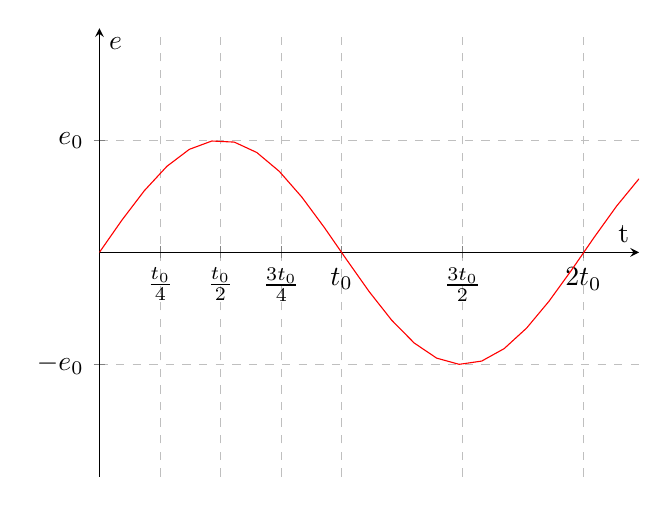
\begin{tikzpicture}
	\begin{axis}[
	    xlabel={t},
	    ylabel={$e$},
	    xmin=0, xmax=7,
	    ymin=-2, ymax=2,
	    xtick={0,0.79, 1.57, 2.36, 3.14, 4.71, 6.28},
	    ytick={-1,0,1},
	    xticklabels={0,$\frac{t_0}{4}$, $\frac{t_0}{2}$, $\frac{3t_0}{4}$, $t_0$, $\frac{3t_0}{2}$, $2t_0$},
	    yticklabels={$-e_0$, 0, $e_0$},
	    ymajorgrids=true,
	    xmajorgrids=true,
	    grid style=dashed,
	    axis lines=middle,
	]
	\addplot[domain=0:7,red] {sin(deg(x))};
	\end{axis}
\end{tikzpicture}\\
\begin{tikzpicture}
	\begin{axis}[
	    xlabel={t},
	    ylabel={$I$},
	    xmin=0, xmax=7,
	    ymin=-2, ymax=2,
	    xtick={0,0.79, 1.57, 2.36, 3.14, 4.71, 6.28},
	    ytick={-1,0,1},
	    xticklabels={0,$\frac{t_0}{4}$, $\frac{t_0}{2}$, $\frac{3t_0}{4}$, $t_0$, $\frac{3t_0}{2}$, $2t_0$},
	    yticklabels={$-I_0$, 0, $I_0$},
	    ymajorgrids=true,
	    xmajorgrids=true,
	    grid style=dashed,
	    axis lines=middle,
	]
	\addplot[domain=0:7,red] {cos(deg(x))};
	\end{axis}
\end{tikzpicture}\\

\begin{align*}
	e &= e_0 \sin(\omega t)\\
	I &= I_0 \cos(\omega t)\\
	s &= s_0 \sin(\omega t)\\
	v &= v_0 \cos(\omega t)\\
	v_0 &= \omega s_0\\
	{\color{bostonuniversityred}I_0} &= {\color{bostonuniversityred}\omega e_0}\\
\end{align*}